\documentclass[12pt]{article}
\usepackage{graphicx}

\usepackage[
backend=bibtex,
style=alphabetic,
sorting=ynt
]{biblatex}
\addbibresource{Manual}

\begin{document}

\newcommand{\pe}{phonon-driver}

\title{User guide to \pe}
\date{2019}
\author{Oto Kohul\'{a}k - pravod@gmail.com}

\maketitle

\tableofcontents

\section{Purpouse}

\subsection{Introduction}
Software package \pe was made to predict structural phase transition in solid state physics. Durring the developent our focus was to make simple python-based object-oriented lightweight easy-to-use program, which after the public release would be licenced under GNU LGPL v 3 licence\cite{GPL}. Code is not a stand-alone work, howewer, it is using various libraries such as ASE\cite{ase-paper} or phonopy\cite{phonopy}\footnote{For more detailed list of dependecies please look at \ref{deps}.}. This document was prepared best intentions, if the read thinks anything is missing please do not hesitate to ask the author or to contribute to the project.

\subsection{Physics behind}

For any defined pressure ($p$) and temperature $T$ thermodynamically the most stable structure ist the one which minimizes the Gibbs potential ($G$):

\begin{equation}
G(X; p, T) = E(X) + pV(X) + TS(X)
\end{equation}

Where $X$ is order parameter\footnote{Any structural parameter which defines the structure.} (in general a multidimenional vector), V is volume of the system and S is the entropy (both as a function of order parameter). In other word the structural parameter which represents the lowest extrem of Gibbs potential is the one thermodynamically stable. If we would move the order parameter of the global minimum a thermodynamic forces would emerge they restore the equillibrium. If we write down the Gibbs potential as Taylor searies the linear therms wanishes:

\begin{equation}
G(X; p, T) = \frac{1}{2}\sum_{i = 1}^N \sum_{j = 1}^N c_{ij} (X_i - X_0) (X_j - X_0) + O(X^3)
\end{equation}

We can focus on quadratic therm $c_{ij}$. Obviously there exist a orthogonal basis set, where the quadratic matric is diagonal. 

At very small or zero temperature ($T = 0K$), the entropy therm can be neglected and from now on we assume that $TS = 0$. At high pressures even energetically less favorable structure can become stable via lower volume. And again, from now on we will focus only on pressure induced phase transitions. If we gradually increase the pressure, we will stay in the same minimum\footnote{Abrupt change may lead to outage from minimum.}. When another thermodynamically favorable minimum appears often it is accopmained with lowering the barrier between these two minima\footnote{See Bell-Evans-Polanyi principle\cite{BEP}.}. This will result in lower eigenvalues of the matrix, which can even become negative (and the minimum will no longer exists). So if we examinate this matrix, which is assosiated with phonon modes we can investigate the possibilities of phase transitions. We have to only carefully increase the pressure and calculate the phonon modes, which are two most fundamental functionalities of our code.


\section{Workflow}

The core element of \pe workflow is the \textit{Pd} object. Is stores every parameter and feature of studied system. When object si initialized (constructed) it assumes all of the settings are alredy stored in the \texttt{settings} directory in separated files (which will be discussed later). One has create this object in python script such as:

\begin{verbatim}
from pd.pd import *

def main():

    START =   0 # kbar
    STOP  = 601 # kbar
    STEP  =  40 # kbar

    runs  = dict ( Aurel = [" "],
                   Local = ["X"]  )

    pd = Pd("Name-of-the-system")

    for Pressure in range(START, STOP, STEP):
        pd.optimize_to_pressure(Pressure, runs)
        pd.prepare_supercell((2,2,2), 0.001, runs)
        pd.calculate_phonons(runs)

if __name__ == "__main__":
    nmc = main()
\end{verbatim}

By invoking the method \texttt{optimize\_to\_pressure}  object will optimize the structure to desired pressure. All of the structural optimizations as well as the fonon calculation are performed by \texttt{VASP}\cite{vasp} package, which employs the DFT theory. However, since \texttt{Pd} uses ASE\cite{ase-paper} driver to comunicate with calculator it is easy to use other calculators as well, such as Quantum ESPRESSO\cite{QE}. Although, this feature has never been tested. All data which were once calculated are stored in SQLite3 database\cite{SQL} therefore if one invokes the optimization to pressure which was already been calculated, the optimization will not occur, instead the precalculated data would be used. The same happend if someone tries to run phonon at some pressure, which has been already calculated. For phonon calculation the phonopy package is used. In the beginnig one has to set the desired supercell dimensions and the displacement for the finited diference method (see the \texttt{prepare\_supercell} method). Finally to calculate phonons one has to invoke \texttt{calculate\_phonons} method.

\subsection{Aurel supercomputer}

Software, which calculats physical quantities, can be executed either on local machine or on supercomputer via \texttt{runvasp.py} script. Detailed description can be optained by executing:

\begin{verbatim}
python3 runvasp.py --help
\end{verbatim}

\subsection{Settings}

In the \texttt{Settings} folder there has to be following files:

\begin{itemize}
  \item \texttt{bands\_settings.py} - contains variables for phonon band structure calculation
  \item \texttt{common\_settings.py} - contains common settings for calculator. If one wants to change energy cutoff for planevawes for every calculation, it can be done either in purpouse specific files or in this one. In the later case it cannot be specified in other files, since it would be overwritten.
  \item \texttt{dos\_settings.py} - contains variables for phonon density of states calculation.
  \item \texttt{ftest\_settings.py} - whenever structural optimization is performed another single point calculation will be performed in order to check the forces. If forces are too big the optimization would be repeatet. In following file settings for this single point calculation are stored.
  \item \texttt{main\_settings.py} - contains main settings like name of the working directory or command for local run of the calculator.
  \item \texttt{opt\_settings.py} - contains optimization specific variables.
  \item \texttt{phpy\_settings.py} - contains phonopy settings.
  \item \texttt{sopt\_settings.py} - After creating a supercell it is important to reoptimize its structure. In this file variables specific to this optimization are stored.
  \item \texttt{xtal\_settings.py} - File where an initial structure has to specified. It has to be in \texttt{ase.Atoms} object or in compatible one.
\end{itemize}

\subsection{Dependecies}\label{deps}

The most important dependecies are listed here:

\begin{itemize}
  \item any OS (Linux, Mac OS, Windows) which supports python3
  \item phonopy library
  \item ASE library
  \item pyspglib
  \item numpy library
  \item virtualenv library (recommanded)
  \item matplotlib library (recommanded)
  \item virtualenv library (recommanded)
\end{itemize}

For complete list of package dependecies as well as their required versions please look at the \texttt{requirements.txt} file in root directory of the package. 

\subsection{Installation}

Package is stored on local gitlab server:
\begin{verbatim}
https://gitlab.mtf.stuba.sk/kohulak/phonon-driver
\end{verbatim}
After one downloads the package it is ready to use. Package contains proper \texttt{setup.py} file for correct integration to other projects. Binary files are in \texttt{bin} directory while library files are in \texttt{pd} directory. It is recomanded to use the package in virtual environment.

\section{Examples}

In order to run an example one has to download the driver. The easiest way is to donwload in via git:

\begin{verbatim}
git clone https://gitlab.mtf.stuba.sk/kohulak/phonon-driver.git
\end{verbatim}

One has to be sure he has all of the necessary dependecies:

\begin{verbatim}
cd phonon-driver

# Following two line can be omited 
# if it not desired to work in virtual environment
python -m venv .
source bin/activate

pip install -r requirements.txt
\end{verbatim}

Recommended way to prepare a calculation is to edit an existing example. For this purpouse \texttt{mkpdexample} script was made:

\begin{verbatim}
mkpdexample [-h] [-F FOLDER] {cuo-nacl,ge}
\end{verbatim}

So far only two examples were made (Germanium and CuO-NaCl).

\subsection{Germanium}

In the beginnig one can prepare the calculation by executing:

\begin{verbatim}
mkpdexample ge -F My-super-ge-example
\end{verbatim}

The folder \texttt{My-super-ge-example} is now containing all of the necessary files. In the root folder there is only one file \texttt{run.py}, which contains work flow:

\begin{verbatim}
from pd.pd import *

def main():

    START =   0 # kbar
    STOP  = 601 # kbar
    STEP  =  40 # kbar

    runs  = dict ( Aurel = [" "],
                   Local = ["X"]  )

    pd = Pd("Ge-diamond")

    for Pressure in range(START, STOP, STEP):
        pd.optimize_to_pressure(Pressure, runs)
        pd.prepare_supercell((2,2,2), 0.001, runs)
        pd.calculate_phonons(runs)

if __name__ == "__main__":
    nmc = main()
\end{verbatim}

Variables \texttt{START, STOP, STEP} defines pressure at which the phonon calculation will be performed. Dictionary \texttt{runs} selects either local run or run on Aurel supercomputer.

In \texttt{settings} folder there are following files:

\begin{verbatim}
bands_settings.py:
settings = { "path"    : "GX", # Band path for phonon disp.
             "npoints" : 100   # number of points on the path
           }

common_settings.py:
# Common settings for vasp calculator
# If variables would not be overwritten
# in other files these settings will be used.       
settings = { "lscalapack" : False,  
             "lwave"      : False,
             "istart"     : 0,
             "encut"      : 250,
             "kpts"       : (3,3,3),
             "nsw"        : 100,
             "nelmin"     : 4
           }
           
dos_settings.py:
settings = { "kpts"        : (21,21,21), # Mesh for phonon
                                         # density of states
                                         # calcualtion
             "tetrahedron" : True        # Use tetrahedron method
           }

ftest_settings.py:
# Vasp settings for force check calcualtion        
settings = { "ibrion"     : -1,
             "nsw"        : 1,
             "ediff"      : 1.0e-6,
           }
           
main_settings.py:
settings = { # Execution directory:
             "vasp_wd" : "calc",
             # Command for local run:
             "locrun"  : "mpirun -np 6 vasp",
             # Command for execution on Aurel superecomputer:
             "aurrun"  : "/path/to/runvasp.py" + \
                         " -c testing -l 1:00:00 -v 5.4.4",
             "dummny"  : None # Deprecated
           }
          
opt_settings.py:
Vasp settings for local optimization:
settings = { "ibrion"     : 2,
             "isif"       : 3,
             "nsw"        : 100,
             "ediff"      : 1.0e-6,
             "ediffg"     : 1.0e-4
           }
           
phpy_settings.py:
# Settings for phonopy:
settings = { "h_step"        : 0.02,         #\AA
           }

sopt_settings.py:
Vasp settings for optimization of the supercell:
settings = { "ibrion"     : 1,
             "isif"       : 3,
             "nsw"        : 100,
             "ediff"      : 1.0e-6,
             "ediffg"     : 1.0e-4
           }
           
xtal_settings.py:
# python script to generate initial structure:
import numpy as np
from ase.io import read
from ase    import Atoms

a = 5.504

# One car easilly set various paremeter like constraints
# or magnetic moments:
settings = {"symbols"          : (['Ge'] * 8),
            "cell"             : np.diag((a, a, a)),
            "scaled_positions" : [(0, 0, 0),
                                  (0, 0.5, 0.5),
                                  (0.5, 0, 0.5),
                                  (0.5, 0.5, 0),
                                  (0.25, 0.25, 0.25),
                                  (0.25, 0.75, 0.75),
                                  (0.75, 0.25, 0.75),
                                  (0.75, 0.75, 0.25)]
           }

# Structure has to be stored in settings variable as ase.Atoms object
settings = Atoms(**settings)

# Alternative way to read structure is from file:

from ase.io import read
settings = read("INIT.POSCAR")

\end{verbatim}

The calculation is started by executing the \texttt{run.py} script. Code will generate the database file, which can be checked as an ase database:

\begin{verbatim}
ase db Ge-diamond.db
\end{verbatim}

In the first few columns one can find the most basic information about performed calculations, such as which calculator was used the maximum force at the end of calculation, energy or volume of the system:

\begin{verbatim}
id| age|user    |formula|calculator|  energy| fmax|  volume|...
 1|216m|kohulako|Ge8    |          |        |     | 166.738|...
 2|216m|kohulako|Ge8    |vasp      | -35.734|0.000| 194.011|...
 3|213m|kohulako|Ge64   |vasp      |-287.448|0.000|1552.091|...
 4|207m|kohulako|Ge64   |vasp      |-287.446|0.201|1552.091|...
 5|207m|kohulako|Ge8    |vasp      | -35.601|0.000| 182.829|...
 6|204m|kohulako|Ge64   |vasp      |-286.476|0.000|1462.636|...
 7|199m|kohulako|Ge64   |vasp      |-286.474|0.233|1462.636|...
 8|199m|kohulako|Ge8    |vasp      | -35.294|0.000| 174.292|...
 9|196m|kohulako|Ge64   |vasp      |-284.021|0.000|1394.335|...
10|191m|kohulako|Ge64   |vasp      |-284.019|0.262|1394.335|...
Rows: 10
Keys: Basic, Displaced, Initial, Pressure, SpaceGroup, Supercell

\end{verbatim}

In later columns we can find another interesting data. We can see that the first row represents the first structure imported from the \texttt{xtal\_settings.py}. Keyword \texttt{Basic} shows that the structure is optimized and not a supercell. Pressure is really self-explanatory and the value is in kilobars. Two keywords \texttt{Displaced} and \texttt{Displnumb} say if the structure was displaced for the phonon calculation a which number of displacement it is. In higly symetric structure, as diamond really is, only one displacement is necessary (counting from zero). Last column shows the spacegroup of the structure.

\begin{verbatim}
id|...|Basic|Initial|Pressure|Supercell|Displaced|Displnumb|SpaceGroup
 1|...|     |   True|        |         |         |         |           
 2|...| True|       |       0|         |         |         |Fd-3m (227)
 3|...|     |       |       0|     True|    False|         |Fd-3m (227)
 4|...|     |       |       0|     True|     True|        0|           
 5|...| True|       |      40|         |         |         |Fd-3m (227)
 6|...|     |       |      40|     True|    False|         |Fd-3m (227)
 7|...|     |       |      40|     True|     True|        0|           
 8|...| True|       |      80|         |         |         |Fd-3m (227)
 9|...|     |       |      80|     True|    False|         |Fd-3m (227)
10|...|     |       |      80|     True|     True|        0|           
Rows: 3
Keys: Basic, Displaced, Initial, Pressure, SpaceGroup, Supercell

\end{verbatim}

After the calculation one can generate and look at the phonon spectra:

\begin{verbatim}
plot_bands Ge-diamond.db
\end{verbatim}

In folder \texttt{figures} the figures will be stored for every pressure which was calculated as it can be seen in Fig. \ref{ge:bands}. One can assume that the pressure induced phase transition occurs between 24 and 28 GPa. Evolution of phonon states at given point can be ploted by executing:

\begin{verbatim}
plot_point Ge-diamond G
plot_point Ge-diamond X
\end{verbatim}

These evolutions can be seen in Fig. \ref{ge:point}. There are two other utilities:

\begin{itemize}
  \item \texttt{showphonon} - Utility to create a displaced super cell according to selected phonon mode.
  \item \texttt{savephonon} - Read and save phonopy data from database.
\end{itemize}

\begin{figure}
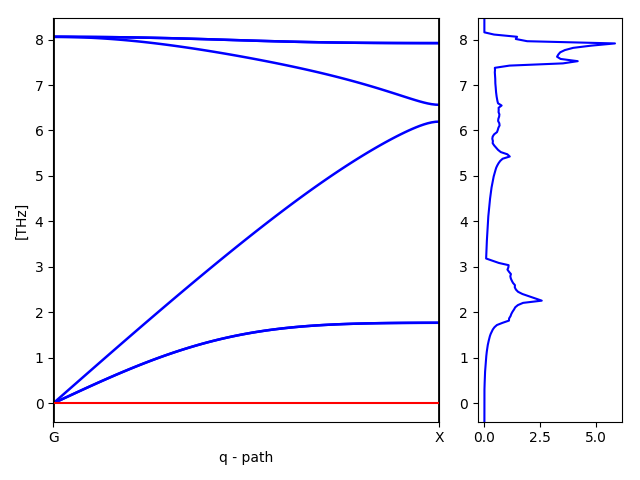
\includegraphics[width=0.5\textwidth]{{figures/name.bands.00000}.png}%
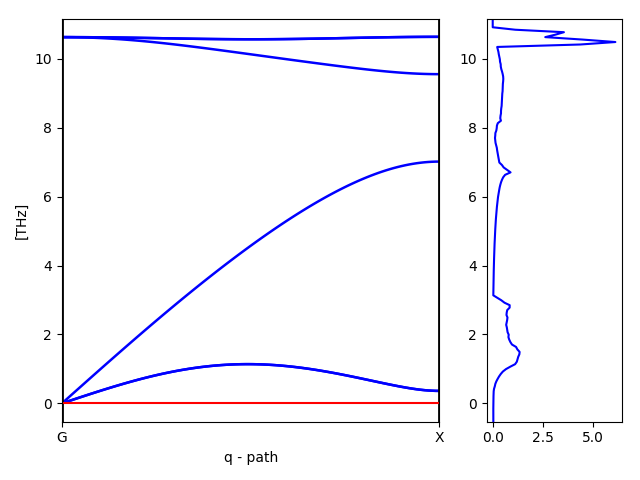
\includegraphics[width=0.5\textwidth]{{figures/name.bands.00240}.png}\\
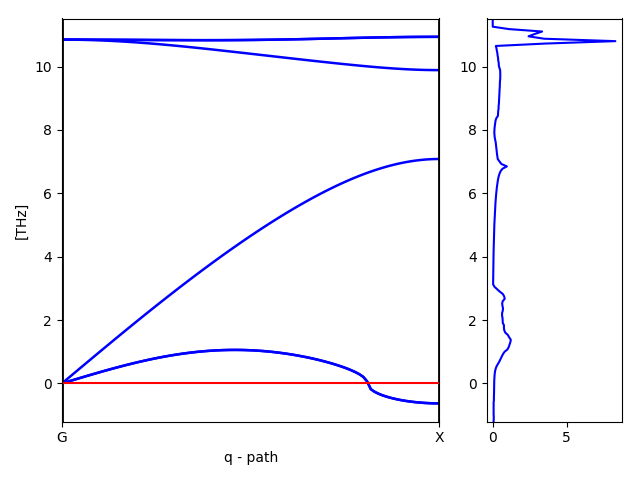
\includegraphics[width=0.5\textwidth]{{figures/name.bands.00280}.png}%
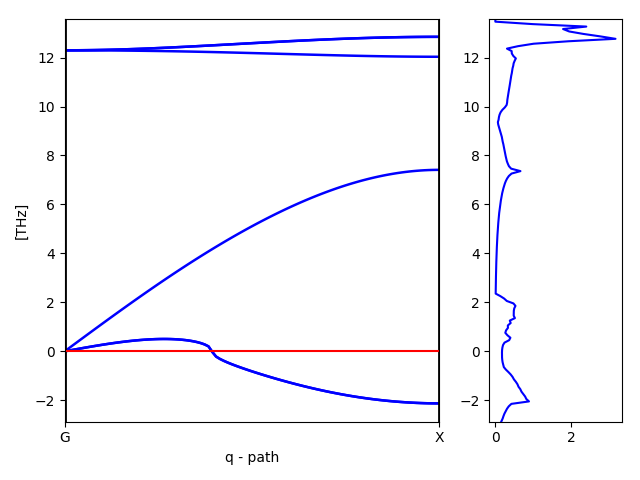
\includegraphics[width=0.5\textwidth]{{figures/name.bands.00600}.png}\\
\caption{On top left subfigure is the phonon band structure (as well as density of phonon states) at zero pressure between G and X point in germanium (diamond structure). On top right is the same disperion at 24 GPa (the highest pressure without imaginary phonons). On bottom left subfigure the pressure is 28 GPa, we can also notice the imaginary phonons. At bottom right are the last disp. relation at highest pressure 60 GPa.}
\label{ge:bands}
\end{figure}

\begin{figure}
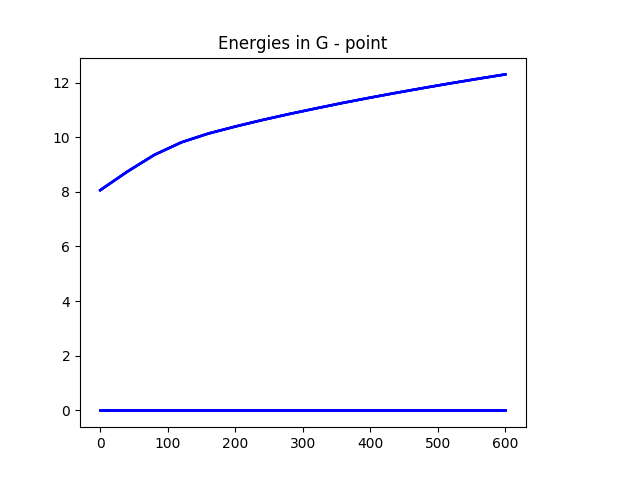
\includegraphics[width=0.5\textwidth]{{figures/name.point-G}.png}%
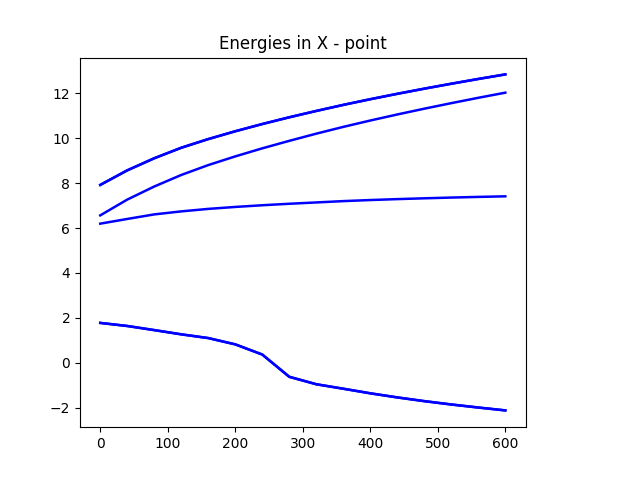
\includegraphics[width=0.5\textwidth]{{figures/name.point-X}.png}\\
\caption{Pressure evolution of phonon states at $\Gamma$ point (left) and $X$ point (right) for Germanium in diamond structure.}
\label{ge:point}
\end{figure}

\subsection{CuO - NaCl}

This example can be prepared by:

\begin{verbatim}
mkpdexample cuo-nacl -F My-super-cuo-nacl-example
\end{verbatim}

\printbibliography

\end{document}